\usepackage{amsthm}

\newtheorem{theorem}{Theorem}[chapter]
\newtheorem{lemma}           [theorem] {Lemma}   
\newtheorem{folg}           [theorem] {Folgerung}   

\newtheorem{frage}       [theorem] {Frage}   
\newtheorem{question}       [theorem] {Question}   
\newtheorem{aufgabe}       [theorem] {Aufgabe}   
\newtheorem{exercise}       [theorem] {Exercise}  

\newtheorem{proposition}     [theorem] {Proposition}  
\newtheorem{satz}     [theorem] {Satz}  
\newtheorem{fact}{Fact}
\newtheorem{definition}      [theorem] {Definition} 

\theoremstyle{definition} 
\newtheorem{bemerkung}     [theorem] {Bemerkung}  
\newtheorem{beispiel}       [theorem] {Beispiel}  
\newtheorem{example}       [theorem] {Example}  
\newtheorem*{example*} {Example}  
\newtheorem{notation}       [theorem] {Notation}  
\newtheorem*{Faust}[theorem]{Rule of Thumb}
\newtheorem*{Boxx}[theorem]{Concept}

%\section{Power Series}
Very roughly speaking, power series are ``infinite polynomials''. A~precise definition is the following:
\begin{Definition}{}
Let a~sequence $(a_k)_{k\in\mathbb{N}}$ in $\mathbb{K}$ be given and let $x_0\in\mathbb{K}$. Then the function $f:D(f)\to\mathbb{K}$ defined by the series
\[f(x)=\sum_{k=0}^\infty a_k(x-x_0)^k\]
is called \emph{power series}.\\
The set
\[D(f):=\left\{x\in\mathbb{K}\;:\;\sum_{k=0}^\infty a_k(x-x_{0})^k\text{ is convergent}\right\}\]
is called \emph{domain of convergence}.  The domain of convergence at least includes $x_{0}$ since $\sum_{k=0}^\infty a_k(x_{0}-x_{0})^k=a_{0}$.
\end{Definition}
We have already seen several examples of power series in this chapter.
\begin{example}\label{ex:powser}
\begin{enumerate}[a)]
\item The exponential function is defined via the power series
\[\exp(x)=\sum_{k=0}^\infty\frac{x^k}{k!},\]
i.e., $(a_k)_{k\in\mathbb{N}}=(\frac{1}{k!})_{k\in\mathbb{N}}$ and $x_0=0$. Here $D(f)=\mathbb{C}$.
\item The sine function is defined via the power series
\[\sin(x)=\sum_{k=0}^\infty\frac{(-1)^kx^{2k+1}}{(2k+1)!},\]
i.e., $(a_k)_{k\in\mathbb{N}}=(0,\frac{1}{1!},0,-\frac{1}{3!},0,\frac{1}{5!},0,-\frac{1}{7!},\ldots)_{k\in\mathbb{N}}$ and $x_0=0$.
Again $D(f)=\mathbb{C}$.
\item $\cos$, $\cosh$, $\sinh$ are defined via the power series...
\item The function
\[f(x)=\sum_{k=1}^\infty\frac{(x-1)^k}{k}\]
is a~power series.
\end{enumerate}
\end{example}

Next we characterise the domain of convergence.
\begin{Theorem}[Theorem of Cauchy-Hadamard]
Let a~power series
\[f(x)=\sum_{k=0}^\infty a_k(x-x_0)^k\]
be given. Let
\[r:=\frac1{\limsup\limits_{k \rightarrow \infty} \sqrt[k]{|a_k|}},\]
where we formally define $1/\infty:=0$ and $1/0:=\infty$. Then for all $x\in\mathbb{K}$ with $|x-x_0|<r$ holds $x\in D(f)$. Furthermore,
for all $x\in\mathbb{K}$ with $|x-x_0|>r$ holds $x\notin D(f)$.\\
The number $r$ as defined above is called the {\em radius of convergence}.
\end{Theorem}

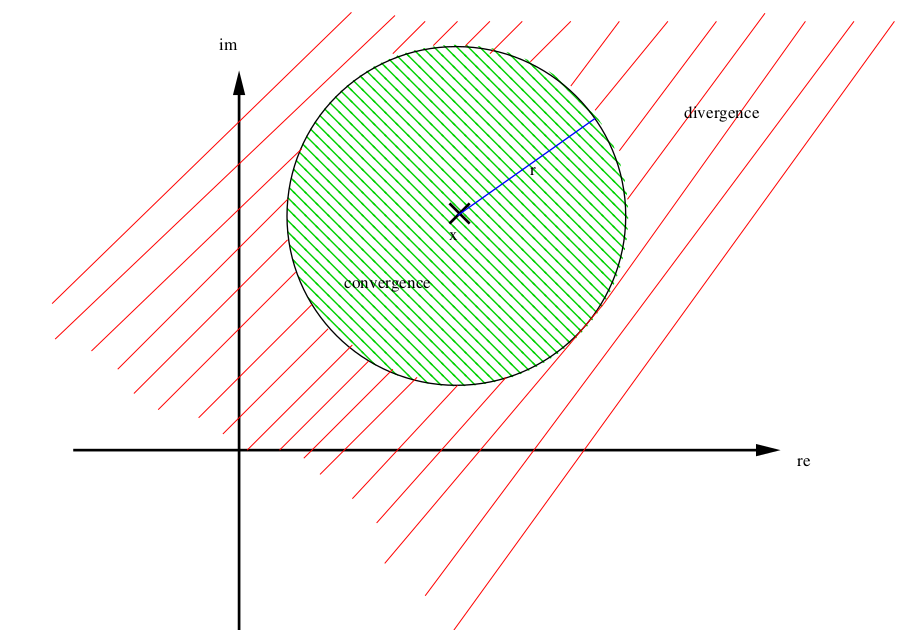
\includegraphics{./power.png}

{\em Proof:} We have to show the following two statements:
\begin{enumerate}[(i)]
\item For all $x\in\mathbb{K}$ with $|x-x_0|\cdot \limsup_{k\rightarrow\infty} \sqrt[k]{|a_k|}<1$, the power series is convergent.
\item For all $x\in\mathbb{K}$ with $|x-x_0|\cdot \limsup_{k\rightarrow\infty} \sqrt[k]{|a_k|}>1$, the power series is divergent.
\end{enumerate}
Statement (i) just follows from the limit form of the root criterion (Theorem \ref{thm:rootkritlim}), namely
\[\limsup_{k \rightarrow \infty} \sqrt[k]{|(x-x_0)^ka_k|}=|x-x_0|\cdot\limsup_{k \rightarrow \infty} \sqrt[k]{|a_k|}<1.\]
\whiteskip
For showing (ii), we also make use of the formula
\[\limsup_{k \rightarrow \infty} \sqrt[k]{|(x-x_0)^ka_k|}=|x-x_0|\cdot\limsup_{k \rightarrow \infty} \sqrt[k]{|a_k|}>1.\]
This implies that the sequence $(x-x_0)^ka_k$ does not converge to 0 and therefore, the power series cannot converge.\hfill$\Box$

Geometrically, the above result implies that for all $x$ inside a~circle with midpoint $x_0$ and radius $r$, 
the series is convergent and outside this circle, we have divergence.\\
The Cauchy-Hadamard Theorem characterizes convergence/divergence of the power series in dependence of $x$ whether it is inside 
or outside the circle around $x_0$ with radius $r$. In the case $|x-x_0|=r$, this result does not tell us anything. Indeed,
we may have points on the circle with $x\in D(f)$ and also points on the circle with $x\notin D(f)$. 

To see this, let us reconsider Example~\ref{ex:powser} d):\\
The radius of convergence is given by
\[r=\frac{1}{\limsup_{k \rightarrow \infty} \sqrt[k]{|\frac1k|}}=1.\]
So we have convergence for all $x\in(0,2)$ and divergence for all $x\in~(-\infty,0)~\cup~(2,\infty)$. 
The remaining real points which are not characterized by the Theorem of Cauchy-Hadamard are $x=0$ and $x=2$. In the case $x=0$, we obtain the series
\[\sum_{k=0}^\infty \frac{(-1)^k}k\]
which is convergent by the Leibniz criterion. Plugging in $x=2$, the power series becomes a harmonic series
\[\sum_{k=0}^\infty \frac{1}k\]
that is well-known to be divergent.
\begin{example}
\begin{enumerate}[a)]
\item For the power series defined by the exponential function, we have \[(a_k)_{k\in\mathbb{N}}=\left(\frac{1}{k!}\right)_{k\in\mathbb{N}},\qquad x_0=0.\]
The radius of convergence is then given by
\[r=\frac{1}{\limsup_{k\rightarrow\infty} \sqrt[k]{|\frac1{k!}|}}=\frac10=\infty.\]
As a~consequence, the series converges for every $x\in\mathbb{C}$. The same holds true for the series of $\sin$, $\cos$, $\sinh$, $\cosh$.
\item As we have already seen above, the radius of convergence of the power series
\[f(x)=\sum_{k=0}^\infty\frac{(x-1)^k}{k}\]
is $r=1$.
\item Consider the power series
\[f(x)=\sum_{k=0}^\infty k! x^k.\]
The radius of convergence is given by
\[r=\frac{1}{\limsup\limits_{k\rightarrow\infty} \sqrt[k]{|k!|}}=\frac1\infty=0.\]
So this series is divergent for any $x\neq0$.
\end{enumerate}
\end{example} 

Sometimes the computation of the radius of convergence $r=\limsup_{n \rightarrow \infty} \sqrt[n]{|a_n|}$ 
of a power series $\sum_{n=1}^\infty a_n(x-x_0)^n$ is quite difficult. In such cases the following theorem might be better suited, 
which follows from the quotient criterion and is stated without proof. 
\begin{Theorem}{}
\label{thm:qutcrit}
	Suppose that $\sum_{n=1}^\infty a_n(x-x_0)^n$ is a power series with coefficients $a_n\in\mathbb{K}$ such that $a_n\neq 0$ for all $n\geq N$ 
  with fixed $N\in\mathbb{N}$. If $\lim_{n\rightarrow\infty} \frac{|a_n|}{|a_{n+1}|}$ exists in $\mathbb{R}\cup\{+\infty\}$ than it is the
  radius of convergence of the power series.
\end{Theorem}

